\section{Discussion}
\label{sec:c3_discussion}

To determine the robustness of our results, and provide clues to the sources of the differences between \arepo\ and \gasoline\ simulations, we ran a number of tests varying code parameters.

\subsection{Resolution Test}
\label{ssec:c3_restest}

%low and high-resolution \arepo\ simulations experience initial mass transfer at about twice the rate of their \gasoline\ counterparts -- the accretion stream is correspondingly denser -- and experience donor disruption at approximately three orbits of the binary, rather than {\gasoline}'s four.  Two factors can contribute to this difference.  First (and based on Sec. \ref{ssec:restest}, perhaps most important), because steep density gradients near the surface of the WDs are treated differently in the two codes, and \arepo\ requires a background grid, stars relaxed in {\gasoline} tend to expand a little when transferred to {\arepo}.  Second, mass transfer in SPH can only occur by passing particles between the WDs, imposing a mass resolution limit, while in \arepo\ no such limitation exists.  This second issue exists even at the highest resolution SPH simulations performed to date, and detailed studies of the accretion stream are best done using a grid code to complement or supplement the SPH simulation \citep{guil+10, ross14}.

As noted in Sec. \ref{ssec:c3_initcond}, an \arepo\ simulation with identical mass resolution to a \gasoline\ one will have roughly a factor of {\charles $3$} higher spatial resolution because of the 100 neighbouring particles needed by the kernel.  It is possible that the differences we observe between our simulations are not due to fundamental differences between the codes, but because our \gasoline\ simulation insufficiently resolves the merger.  To address this, we performed a series of \gasoline\ and \arepo\ simulations with a mass resolutions of $5\times10^{28}\,\mrm{g}$ (equivalent to $5.1\times10^4$ particles/cells and comparable to resolutions used in parameter-space sweeps \citealt{dan+12,dan+14}), $1\times10^{28}\,\mrm{g}$ ($2.6\times10^{5}$) and $1\times10^{27}\,\mrm{g}$ ($2.6\times10^{6}$).  This factor of $50$ range in mass resolution ($\sim4$ in spatial resolution) allows us to both determine the degree to which mergers in each code change with resolution, and to can compare \arepo\ runs to \gasoline\ ones at finer mass resolution.

At all four resolutions, the \gasoline\ simulations exhibit very similar behaviour prior to coalescence.  The donor fully disrupts in at $\sim3.5$ orbits of the initial binary for the two higher resolution runs, while the two lower-resolution ones experience a slightly earlier disruption at $\sim3.2$ orbits ($\sim155-160\,\mrm{s}$).  Coalescence for the highest resolution run occurs at $\tcoal = 230\,\mrm{s}$, within $2$ seconds of the standard resolution value, while it occurs $15 - 30$ seconds earlier for the two lower resolution runs (we note the method we determine coalescence is somewhat sensitive to changes in the detailed configuration of the remnant).  Just after coalescence, all reproduce the crescent-and-void configuration, with the void being least prominent in the lowest-resolution run.  \arepo\ also reproduces the same qualitative evolution up to coalescence at all resolutions, but donor disruption occurs within only $\sim2$ orbits it its lowest resolution, and in $\sim3$ in its second lowest.  The time of coalescence is likewise much sooner in the lowest resolution simulation, at $\tcoal = 150\,\mrm{s}$ for the lowest resolution run.  The two higher resolution runs, however, are very similar to one another, with donor disruption occuring at $\sim180\,\mrm{s}$ and $\tcoal = 234\,\mrm{s}$, much closer to the standard resolution run's values.  These differences are in part due to our initial conditions setup, where \gasoline\ SPH particles are directly mapped to \arepo\ cells.  WDs that are hydrostatic in \gasoline\ are not precisely so in \arepo, particularly in the poorly resolved atmosphere, and we see the WDs spuriously expanding in the first few seconds.  This effect leads to larger mass-transfer rates early in the merger, and is magnified with decreasing resolution.  Just after coalescence, all reproduce the crescent-and-void configuration, with the void being least prominent in the lowest-resolution run.

% Personal note on initial conditions: as described by Agertz et al. 2007 and Hess & Springel 2010, surface tension applies at the interface between two fluids of differing densities but the same pressure.  As particles from the less dense fluid approach the interface, they begin sampling only the density of the denser fluid (since they comprise the majority of nearby particles).  This overestimates incoming particles' densities, leading to an additional repulsive force that inhibits mixing.  I understand the qualitative picture (the SPH equation of motion uses only the density of the local particle, not its mass, so an increase in density is equivalent to an increase in mass, and this becomes a bigger and bigger problem as the particle approaches the interface, thereby reducing accelerations; these accelerations "go back to normal" as the particle moves away).  I'm unable to replicate it in equations though.  I suspect that for hydrostatic equilibrium, what's happening is that particles at the surface of the star will both have spuriously high densities and forces coming from only one side.  The latter is simply a poor estimate, but the former is a systematic offset that will shrink the size of the star and, when we map our SPH initial conditions into Arepo, create systematically high densities in the outermost layers of the star.  This means we're making a star that's missing its outer layers (because SPH doesn't have the mass resolution) and piling that material slightly deeper down in the star.  In Arepo, this would act like a spring, leading to more violent oscillations.  I'm not certain why the final state of the relaxed star in Arepo has lower central density - perhaps because the atmosphere is heated more from the oscillations, the center sees less weight?

% The lowest resolution merger in Arepo also seems to heat a bit more prior to the merger, which might be due to a combination of the hydrostatic equilibrium issue and 

\begin{figure}
\centering
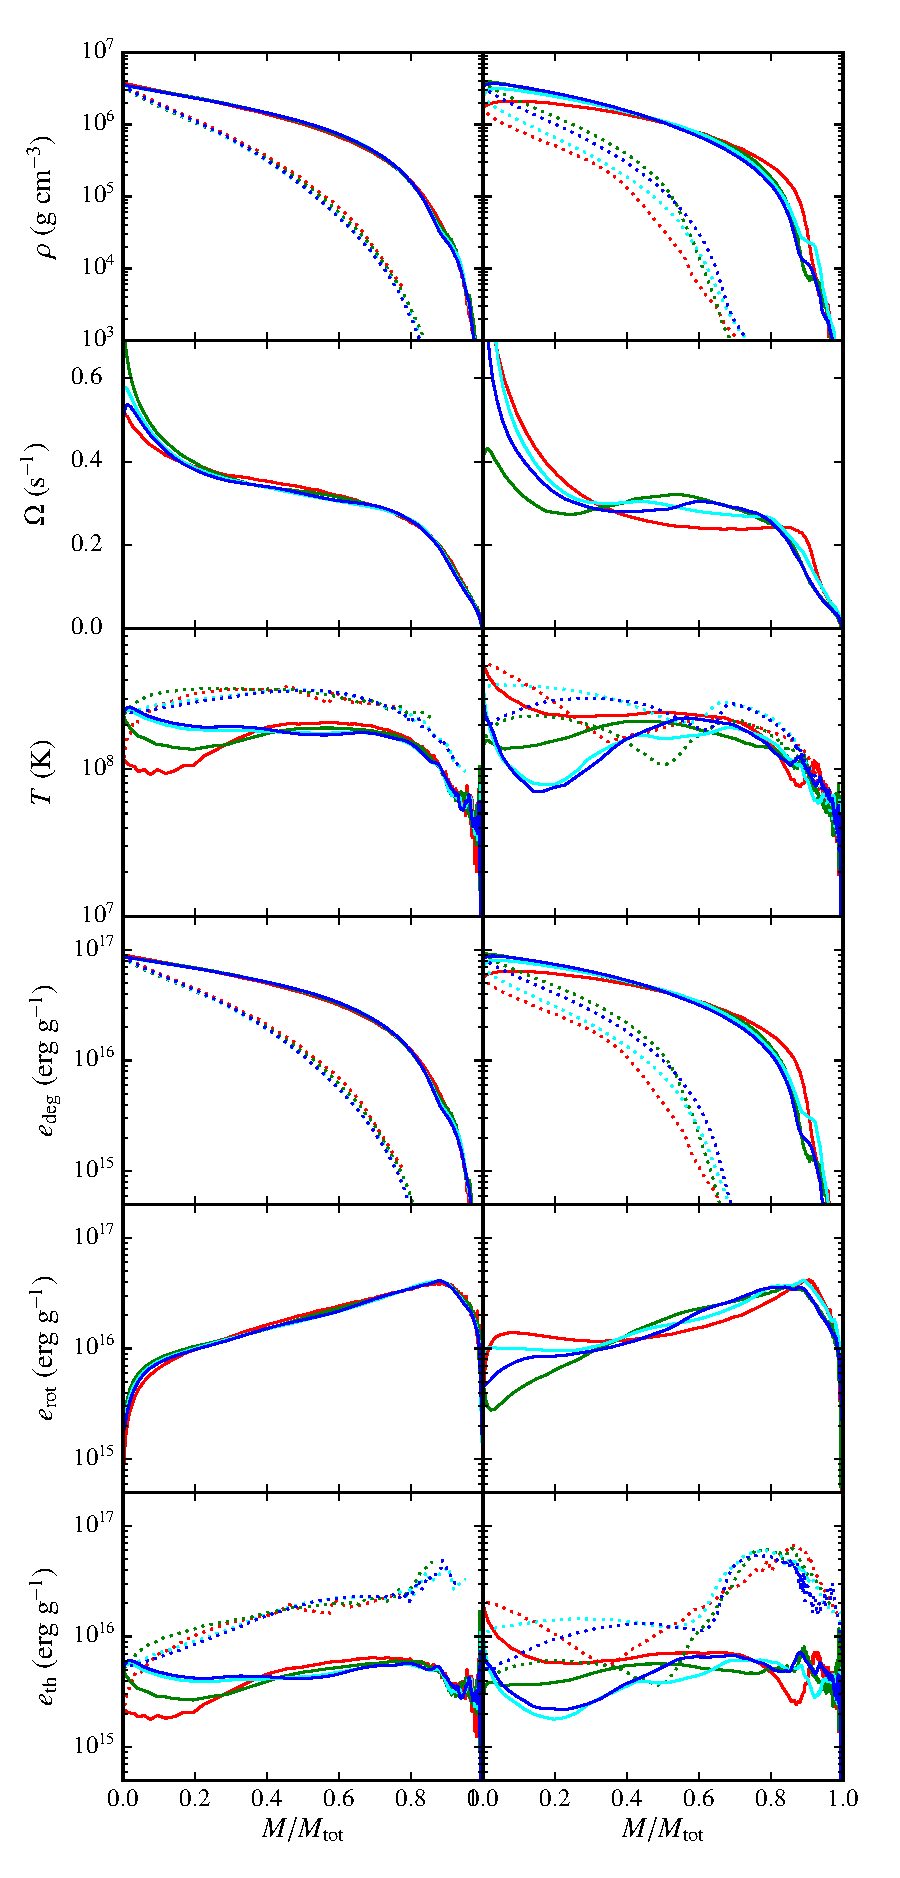
\includegraphics[angle=0,width=0.6\columnwidth]{chapter3_zhu+u/figures/curves_res.pdf}
\caption{Merger remnant profiles, as in Fig. \ref{fig:c3_curves}, for \gasoline\ (left column) and \arepo\ (right) simulations of various (initial, for \arepo) mass resolutions.  Resolutions include $5\times10^{28}\,\mrm{g}$ (equivalent to $5.1\times10^4$ particles/cells; red lines), $1\times10^{28}\,\mrm{g}$ ($2.6\times10^{5}$; green) $2\times10^{27}\,\mrm{g}$ ($1.3\times10^{6}$; cyan) and $1\times10^{27}\,\mrm{g}$ ($2.6\times10^{6}$; blue).}
\label{fig:c3_res_curves}
\end{figure}

In Fig. \ref{fig:c3_res_curves}, we plot the equatorial and rotational axis profiles of all simulations $100\,\mrm{s}$ after their time of coalescence.  The \gasoline\ remnants (left column) are all remarkably similar to one another, with the sole exception of the temperature structure at the lowest resolution.  The disk and core-envelope masses as well as internal energy and its partitioning into various forms are all within $1$\% of their values at standard resolution reported in Sec. \ref{sec:c3_results}.  The central density also deviates by $\lesssim3$\% from $3.6\times10^{6}\,\gcc$ in all remnants.  The \arepo\ remnants (right column) are less uniform: masses and energies vary by $\sim10$\% from their reported values in Sec. \ref{sec:c3_results}, and the central density ranges from $3-4\times10^6\,\gcc$ for all resolutions except the lowest one, where it is $\sim2\times10^6\,\gcc$.  The variations in the rotation and temperature curves reflect variations in the structure of the dense crescent and hot void.  While at the highest two resolutions the dense crescent is clearly colder, with a temperature of $\sim6\times10^7\,\mrm{K}$, at a resolution of $1\times10^{28}\,\mrm{g}$ the crescent's temperature is a much warmer $3\times10^8\,\mrm{K}$, and at the lowest resolution the remnant's core never forms a crescent at all, instead appearing as a dumbbell-shaped object that transforms into a spherically symmetric one within $500\,\mrm{s}$ of coalescence.  During this time, global angular momentum decreases by $\sim10$ (see Fig. \ref{fig:c3_fix_angmo_nar}), and a $<10^7\,\mrm{K}$ ring of material spurious forms at the interface between donor and accretor, both indicating that the \arepo\ is too poorly resolved to simulate the merger.  At all other resolutions, however, the crescent and void survive until the end of the simulation at $1000\,\mrm{s}$.

The crescent-void configuration also appears, but then fades away over several hundred seconds, in all \gasoline\ simulations.  To check if the longevity of the configuration is resolution-dependent, we turn to \citealt{zhu+13}'s measurement of non-axisymmetry, measured from $|f_i|/|f_0|$, the ratio of largest non-zero to zeroth Fourier coefficient of particles or cells binned in azimuth.  For all simulations, the largest non-zero Fourier coefficient is the first, and the time the hot void disappears the remnant roughly matches the time $t_f$ when $|f_1|/|f_0| = 0.01$.  We find, from lowest to highest resolution, $t_f = 425\,\mrm{s}$, $483\,\mrm{s}$, $515\,\mrm{s}$ and $513\,\mrm{s}$ -- roughly corroborated by visual inspection of the remnant's non-axisymmetry -- that suggests convergence at $t_f \approx 510\,\mrm{s}$.   Note that all \arepo\ simulations maintain $|f_1|/|f_0| \gtrsim 0.1$ for $\gtrsim 1000\,\mrm{s}$, except (unsurprisingly) for the lowest-resolution run, which drops to $|f_1|/|f_0| \approx 0.02$ by the end of the simulation.

We thus conclude that the largest difference between the \gasoline\ and \arepo\ simulations -- the survival of the crescent-void configuration long after the merger -- is the case for all resolutions.  The void persists for hundreds of seconds in all but the lowest-resolution \arepo\ simulations, while even in the highest-resolution \gasoline\ one it smears away, disappearing within $\sim 250$ s after coalescence.  This indicates that spatial resolution alone is insufficient to explain the diverging behavior of the codes.  We also find that, curiously, that \gasoline's results change little between all resolutions, while \arepo's results only appear to agree at the highest resolutions.  This bodes well for merger parameter-space studies using lower-resolution SPH simulations (eg. \citeal{zhu+13}, \citealt{dan+14,}; the latter finds in their resolution study similar results unless nuclear burning becomes important during the merger), but the same study would require a mass resolution finer than $\sim1\times10^{28}\,\mrm{g}$ in \arepo\ (and ideally closer to our standard resolution of $2\times10^{27}\,\mrm{g}$) to guarantee qualitative accuracy with higher-resolution runs.

\subsubsection{Varying Viscosity in \gasoline}
\label{ssec:c3_vary_visc}

Artificial viscosity, which is essential in SPH for proper shock capture, has been a major issue for white dwarf merger simulations for decades (eg. \citealt{guerig04, loreig09}) because it spuriously shears differential rotation into rigid rotation, dumping excess energy into heat.  This viscosity cannot simply be mitigated by resolution \cite{spri10rev}, and we cannot run our mergers with zero artifical viscosity without neglecting shock heating and introducing unphysical particle behaviour.  We can, however, increase and reduce its strength to see what effect it has on our simulation results, as in \citeal{zhu+13} {\charles Sec. XXX}.

We ran \gasoline\ simulations of our merger with a mass resolution of $1\times10^{28}\,\mrm{g}$ and time-independent artificial viscosity coefficients of either $\alpha\,=0.05$, $\beta\,=0.1$, or $\alpha\,=1$, $\beta\,=2$ (the Balsara switch is still active), comparing them to the variable-viscosity run at the same resolution in Sec. \ref{ssec:c3_restest}.  These simulations both experience donor disruption after $\sim3.2$ binary orbits, similar to the variable one, and coalescence occurs at $205\,\mrm{s}$ and $219\,\mrm{s}$ for the low and high-viscosity runs, respectively.  This similarity is to be expected, since mass transfer and donor disruption are governed by tidal forces, which are unchanged between the simulations.  During coalescence, the evolution of the variable and high-viscosity runs is similar, except that the accretor becomes about twice as hot.  In the low-viscosity run, however, the donor's accretion stream produces a contiguous hot ring around the accretor during coalescence, rather than the string of vortices seen in row 2 of Fig. \ref{fig:c3_diag}, and perturbes the accretor far less.  As a result, no distinct void ever forms, though the remnant core is distorted into a bean shape.  Within $\sim25\,\mrm{s}$ of coalescence, the void in the high-viscosity simulation is already fast-disappearing, having a radius less than half of that of the variable-viscosity run.  $t_f = 358\,\mrm{s}$ and $486\,\mrm{s}$ for the high and low-viscosity runs, respectively, compared to $483\,\mrm{s}$ for the variable one.  The similarity of the latter two values is likely because the variable-viscosity run tends toward the same $\alpha$ and $\beta$ values as the low-viscosity one in the absence of shocks.  At $\sim500\,\mrm{s}$, the remnant has become axisymmetric in all three codes, but in the high-viscosity run the interior $\sim0.8\,\Msun$ of the remnant is also rigidly rotating with $\Omega = 0.33\,\mrm{s}^{-1}$, and features a nearly uniform temperature of $2 - 2.5\times10^8\,\mrm{K}$. 

As expected, then, the high-viscosity simulation rapidly spins down to axisymmetry while eliminating differential rotation, showing that excess artificial viscosity contributes to the disappearance of the crescent-void configuration.  The low-viscosity simulation, on the other hand, primarily shows the importance of increasing $\alpha$ and $\beta$ during coalescence in order to properly capture shocks and shearing interactions between donor and accretor.

% Void sizes use the DENSITY intensity maps, not temperature.

%\subsubsection{Differences in the Merger Process}
%\label{ssec:c3_differences_merger_process}

%%NOTE TO SELF: a greater temperature differential may NOT mean that much if the difference in specific energies is nearly the same!  I still need to check this.  It would also be good to include something about the specific rotational energy of the void, and whether or not overall the low-viscosity run is more rotationally supported.

%%\lanza 10 a attempt to mitigate artificial viscosity by, and \lanza 10 replaced artificial viscosity in the SPH momentum and energy equations with an equation of state that captures the increase in pressure due to physical dissipation.  Tests using these modifications show much stronger accretion disk spiral waves than equivalent standard SPH simulations.

%%COMMENT: The papers cited above are annoyingly hard to read.  In lanza 10 b, the general implementation of the EOS results in an accretion ring rather than a disk.  Lanzafame cites this as being because physical dissipation is necessary for maintaining an accretion disk.


%The disappearance of the hotspot in \gasoline\ could have a number of causes: viscosity, spatial resolution, differences in merger structure at coalescence, and SPH surface tension.

%The primary differences between the \gasoline\ and \arepo\ simulations arising from the merger up to coalescence include a much earlier and faster mass transfer phase (which we cannot rule out as being an initial conditions effect), a more disrupted accretor (leading to a more cresent-shaped remnant core) and a more prominent, faster-spinning low-density void near the middle of the remnant.

%Differences are to be expected, as the merging process involves steep gradients of both density and temperature, shocks from direct impact accretion and and supersonic shear flows mixing with each other, all of which are taxing on hydrodynamic codes.  Our \gasoline\ simulations have poorer spatial resolution than our \arepo\ simulations, and therefore should have a harder time capturing steep gradients, and artificial viscosity, even if adaptive, may be insufficient to properly treat a region containing both shocks and shear flows.

%We do not that our high-resolution \gasoline\ remnant better approximates our \arepo\ results than our low-resolution \gasoline remnant - the remnant core's shape is quite similar at either resolution, both being denser and less cresent-shaped than the core in either \arepo\ simulation.  We did not perform a \gasoline\ simulation at comparable spatial resolution to our \arepo\ simulations to the computational demand of such a simulation.  

%As an additional check of \arepo's veracity, we ported \arepo's initial conditions to the Eulerian grid code \flash\, operating with a fixed grid that has higher resolution close to the remnant core.  The post-coalescence evolution in \flash\ initially qualitatively resembled that of \arepo, but angular momentum transport was much slower.  After XXX s, the transport damped away.  If we freeze \arepo's mesh-generating points in space (reducing \arepo\ to a second-order Eulerian code on an irregular grid), we find a strikingly similar remnant evolution.  A close examination of the remnant core's shape shows that, in both \flash\ and static-grid \arepo, instead of evolving from a cresent-shaped object into a bar, before becoming spherical, the void simply shrinks over XXX s, as if the cresent's structure was being smeared out.  This is consistent with the increased diffusivity of fixed grid codes compared to moving mesh, and similar to the effect of artificial viscosity on the remnant core in \gasoline, making moving mesh \arepo\ the only set of simulations that does not artificially smear the core into axisymmetry.

%In both \gasoline\ and in \arepo\ the void has a lower pressure than its surroundings, even when including rotational support, but the accretor material around it has high specific angular momentum, which needs to be transported away before the accretor can fill the void.  

%%COMMENT: should we be looking at a resolution test of fixed-grid Arepo?  How about a resolution test of FLASH, so that we find that for increased resolution, angular momentum transport increases in magnitude/lasts longer before damping out

%%We also tried transplanting a late-time Gasoline frame into Arepo, but this ALSO resulted in angular momentum transport.  It's difficult to discern where this transport is coming from - small, stubby high-order wave modes appear in the simulation, but the entire system appears to suffer from spurious angular momentum transport.  Because there is no off-centre component to the remnant, I can only imagine this is a resolution problem.

%\subsection{Post-Merger Evolution and Spurious Angular Momentum Losses}
%\label{ssec:pmeloss}

%%High res Arepo 50% loss frame:  502
%%Low res Arepo 50% loss frame:  439
%%No volume hack high res Arepo 50% loss frame:  432
%%No volume hack low res Arepo 50% loss frame:  292
%%For High res Arepo , loss is from  1.85189628455e+50 to 9.09809608812e+49
%%Total Lz loss is from 3.89615927037e+50 to 3.50546713226e+50 41.4709334267 % of inner Lz lost and 10.0276223584 % of total Lz lost
%%Total balance loss is from 1.85189628455e+50 to 1.49778987145e+50 37.5874558268 % of inner Lz lost
%%For Low res Arepo , loss is from  1.92422726705e+50 to 9.50364582136e+49
%%Total Lz loss is from 3.89705830009e+50 to 3.31924980397e+50 59.3316188274 % of inner Lz lost and 14.8267860428 % of total Lz lost
%%Total balance loss is from 1.92422726705e+50 to 1.47318235503e+50 46.3150420493 % of inner Lz lost
%%For No volume hack high res Arepo , loss is from  1.80999272769e+50 to 8.89213851496e+49
%%Total Lz loss is from 3.89617313125e+50 to 3.20548831733e+50 75.0109316992 % of inner Lz lost and 17.7272618709 % of total Lz lost
%%Total balance loss is from 1.80999272769e+50 to 1.23560208983e+50 62.3809529855 % of inner Lz lost
%%For No volume hack low res Arepo , loss is from  1.933334036e+50 to 9.56927199237e+49
%%Total Lz loss is from 3.8971170875e+50 to 3.10551669593e+50 81.0728030329 % of inner Lz lost and 20.3124610781 % of total Lz lost
%%Total balance loss is from 1.933334036e+50 to 1.28752907697e+50 66.1409706198 % of inner Lz lost

%Spiral waves has long been cited as a means for transporting angular momentum in accretion disks (\citealt{balb03} and references therein), in particular to accrete material from a disk onto a star or compact object (eg. \citealt{sawamh86}, \citealt{savopl94}) and facilitate the inward migration of terrestrial planets (eg. \citealt{kleyn12}).  Past simulations have shown that, similar to our case, SPH tends to suppress the expected formation of spiral waves.

%\cite{dval+06} performed an extensive battery of tests on 17 independent codes, 15 Eulerian and 2 SPH, simulating in two dimensions a planet on a circular orbit interacting with a protoplanetary disk.  The planet is expected to tidally excite a spiral wave from each of its two Lindblad resonances and open a density gap in the disk.  The Eulerian codes all reproduced these broad features as well as a number of non-linear ones such as vorticies at the, and their azimuthal and radial density profiles broadly agreed in shape - in many cases they numerically agree to within a few percent \textbf{check with pavel?}.  The SPH codes, on the other hand, produce gaps with poorly resolved boundaries (or in the case of shallow gaps, a poorly resolved gap in its entirety) and highly diminished spiral waves.  SPH density density profile had both different shapes and substantial systematic offsets.  Consequently, the tidal torques between the sprial waves and the planet measured by the Eulerian codes was far stronger than the torques measured by the SPH codes.  \cite{dval+06} speculated these differences were due to the diffusive nature of SPH, as well as code features like the Balsara switch designed to reduce viscosity in shear flows also leading to poor shock capture in those same regions.

%Artificial viscosity has long been cited as hindering the formation of spiral shocks under conditions theoretically favourable to their production (ex. \citealt{yukabm97, lanzb97, lanz03}).  In particular, sprial waves more readily develop in 2D disk simulations than in 3D due to the reduced effect of artificial viscosity in 2D \citep{lanz03}.  \cite{lanz10} attempts a more physically realistic implementations of artificial viscosity, and find stronger spiral waves develop in accretion disks as a result.

%%Both \citeauthor{dval+06} and \cite{hubbfg13} find the development of fine features such as instabilities can be captured as well as grid codes if a comparatively higher spatial resolution is used, but this is computationally prohibitive in our case.

%Moreover, the remnant core's peanut structure and its surroundings are in no way rigidly rotating, and a strong artificial viscosity quickly drives the remnant toward axisymmetry.  An axisymmetric core cannot drive waves through either tides or ram pressure, so artificially smearing out peanut also suppresses angular momentum transport.  We find that the $\alpha\,=1$, $\beta\,=2$ fixed viscosity \gasoline\ test run has the core reach axisymmetry at around XXX s after coalescence, $\sim50$ s faster than our production run and XXX s faster than our $\alpha\,=0.05$, $\beta\,=0.1$ fixed viscosity test.  Artificial viscosity therefore damps both the driving and transport of waves.

%In Fig. \ref{fig:resangmo} we again plot the inner angular momentum, this time for our low and high-resolution \arepo\ simulations, and also plot ones with the same low and high-resolution initial conditions, but without the explicit refinement criterion.  Also plotted, in dashed lines, are the total angular momenta of the four simulations over time, shifted downward vertically by $1.5\times10^{10}$ g cm s$^{-1}$ to directly compare with inner angular momentum losses.  Due to our refinement criteria, all of our \arepo\ simulations, including those without the explicit criterion, increase in resolution over time.  To compare the different simulations, we use \Ntavg\, the number of mesh-generating points time-averaged over the entire duration of a simulation.  Our high resolution simulation has $\Ntavg = XXX$, our low resolution $\Ntavg = XXX$, our high resolution simulation without explicit refinement has $\Ntavg = XXX$, and low resolution without explicit refinement $\Ntavg = XXX$.

%Higher resolution simulations spin down more slowly than their low resolution counterparts, and the spin down ends when the core has more angular momentum remaining.  The loss curves for all of these simulations is very similar except for the high-resolution production run.  All simulations pass through the same qualitative stages of the spin-down -- single spiral wave from a cresent-shaped object transforming to two waves generated by a bar -- except the other three simulations experience a smoother evolution from crescent to bar, with no temporary loss in spiral wave strength, than high-resolution production run (Sec. \ref{ssec:postmergerevo}).  On the other hand, spurious angular momentum losses are reduced almost by a factor of three when going from lowest to highest resolution.

%Fig. \ref{fig:restest} shows the relationship between time-averaged resolution and fraction of total angular momentum at $t_\mathrm{50\%}$, the time when \Lzinner\ has been reduced to 50\% its maximum value ($t_\mathrm{50\%}$ is larger for higher-resolution simulations because they have slower spin-down).  A logarithmic best fit is also plotted, and has the functional form

%\eqbegin
%\frac{\Delta \Lztot}{\Lztot(t=0)} = -0.034\Ntavg + 0.684
%\label{eq:restestfit}
%\eqend

%\noindent This indicates an extremely slow convergence -- $\Delta \Lztot /  \Lztot(t=0)$ reduces to below 0.01 only when $\Ntavg > 3\times10^8$.    Fig. \ref{fig:restest} also shows that having an explicit refinement criterion like we did is important in reducing spurious angular momentum losses, but only because it dramatically increases the total resolution of the simulation.  Utilizing extremely high resolutions in our initial conditions, or artificially increasing the resolution after coalescence, would likely produce similar results (though perhaps requiring more computational resources).

%To better poinpoint where in the system the angular momentum is being spuriously lost, we performed a calculation, similar to \cite{ji+13} Sec. 2.2.4, to determine the amount of theoretically expected angular momentum transport.  If a fluid is inviscid, then from Euler's Equation the conservation of angular momentum is

%\eqbegin
%\frac{\partial L_i}{\partial t} = - \oint_V \epsilon_{ijk} \rho x^ju^k u_l dl^l + \int_V \epsilon_{ijk} x^j F^k dV - \int_V \epsilon_{ijk} x^j \partial^kP dV
%\label{eq:angmobalance}
%\eqend

%\noindent where the first term is advective, the second external torque and the third pressure torque.  We use this equation to calculate the theoretical inner angular momentum \Lzinner\ as a function of time, and find the discrepancy between the theoretical and simulation \Lzinner\ is greater than 80\% of the total spurious angular momentum loss for all our simulations.  By the time $t_\mathrm{50\%}$ is reached, about two-thirds of \Lzinner\ was lost spuriously in the low-resolution simulation without explicit refinement, and $\sim35$\% of \Lzinner\ is spuriously lost for our high-resolution, explicitly refined simulation.  Just inside $10^9$ cm is the interface between the high density core and surrounding envelope features, which features large density gradients and shearing, vorticies, and other complex fluid flows.  These features may be why our simulations, including the \gasoline\ 503 s snapshot transplanted into \arepo\ mentioned in the previous section, are prone to lose angular momentum here instead of in the core and outer disk, which have much more regular bulk motion.  This may also be why spurious angular momentum losses are negligible before coalescence, as the core-envelope interface has not yet formed.

%We cannot truly make spurious angular momentum losses negligible without going to prohibitively costly resolutions, and they affect all our simulations.  At the same time, spiral waves are physically expected due to the non-axisymmetry of the remnant just after coalescence, and from our theoretical angular momentum calculations, comprise the majority of the angular momentum loss observed in the simulation.  Our merger remnants all spin down to near-axisymmetry with one, then two, spiral waves regardless of resolution.  We therefore believe that the qualitative features of post-merger evolution are robust, while the timescale and exact amount of angular momentum left following spin-down being resolution-sensitive.

%Angular momentum conservation issues were not reported in other \arepo\ and SPH code comparisons, notably among them the large-scale structure formation simulations of \cite{voge+12} and galaxy mergers of \cite{hayw+13}, both of which develop disk strutures.  \cite{hayw+13} only simulate isolated disk galaxies for a few dozen dynamical times, an order of magnitude less than in our simulations, and then simulate their merger over several dozen additional dynamical times with star formation and supernovae feedback included.  \cite{voge+12} performs simulations spanning hundreds of dynamical times, but their simulations feature radiative cooling, a time-dependent ionizing UV background and stellar evolution embedded within an expanding FLRW universe.  Both codes have long-range forces dominated by dark matter.  Due to these fundamental differences in dynamical times simulated and physics included, we cannot conclude whether the lack of global angular momentum conservation also affects these other works.

%\textbf{Ruediger, I think we should mention a few other Arepo-only simulations here (Federico's stuff?), and why they don't necessarily suffer from spurious angular momentum losses.  What do you think?}

%\subsection{Ramifications for Merger Outcomes}
%\label{ssec:ramifications}

%Our current studies somewhat affect the conclusions made for pre-coalescence merger evolution made in other works.  A number of previous works (DAN, RASKIN, RUEDIGER?) use relatively low-resolution SPH simulations to try to discern if helium or carbon will violently ignite during the early stages of mass transfer.  As we find higher temperatures in newly accreted material during this phase of the merger, we believe that SPH may underestimate the potential for violent nuclear reactions.  This has been long-suspected, and is the reason why \cite{guil+10} used a hybrid approach to simulate early mass transfer during a merger.  As shown in Fig. \ref{fig:comp}, the bulk properties and overall profiles between \arepo\ and \gasoline\ are similar, except for the low-density void near the remnant core centre and a much lower core temperature.  We performed a number of low-resolution diagnostic tests which show that, even for an unsynchronized, nearly equal-mass 0.625 - 0.626 \Msun\ merger, the merger remnant remains centrally cold, surrounded by a warmer envelope, in contrast to our SPH results in \citeauthor{zhu+13}, as well as \citeauthor{loreig09}.

%The more impactful change to the conclusion of other works we make is that hydrodynamic evolution does not stop at coalescence, and a spiral wave-mediated spin down of the merger remnant occurs over several thousand seconds.  This spin-down originates from the non-axisymmetry of the remnant core, which itself originates from material from the tidally destroyed donor impacting the accretor.  Merger remnants of dissimilar-mass mergers will experience far less accretor disruption than the system we present here, but we find for a low-resolution 0.5 - 1.0 \Msun\ CO WD merger that the \textit{donor} does not disrupt into a completely axisymmetric disk around the accretor, and this non-axisymmetry powers a spiral wave propagating into the disk.  Hydrodynamic spin down is therefore likely prevalent throughout the majority of the WD merger parameter space.

%Because previous works found hydrodynamic evolution to stop at coalescence, it was expected that the next phase of evolution for the remnant would be a magnetically-driven spin-down phase lasting of order hours to days \citep{vkercj10, shen+12}.  \cite{schw+12} and \cite{ji+13} have both simulated this evolution by porting SPH merger results into 2.5D hydrodynamic simulations.  \citeauthor{schw+12} use \textsc{zeus-mp2} fitted with the Helmholtz EoS, a \cite{shaks73} shear viscosity set to $\alpha = 3 \times 10^{-2}$ and a five-isotope nuclear network in order to evolve merger remnants imported from \cite{dan+11} with a span of masses and compositions.  For their fiducial 0.6 - 0.9 \Msun\ remnant, they find it nearly completely spins down over $3\times10^4$ s, transferring its disk mass and most of its angular momentum into a thermally supported thin envelope (the remnant core barely changes in mass).  The material at interface between core and disk, where there is a temperature peak, is compressed by loss of rotational support such that its temperature increases from $5\times10^8$ K to $7.5\times10^8$ K, and its density from $2\times10^5$ \gcc\ to $6\times10^5$ \gcc.  Very little mass is lost.  \citeauthor{ji+13} use \flash\ in AMR mode to simululate the full magnetohydrodynamic evolution of a 0.6 - 0.6 \Msun remnant ported from \citeauthor{loreig09} and augmented with a weak poloidal seed magnetic field.  Over $2\times10^4$ s, the remnant core loses 70\% of its angular momentum, the magnetic field strengthens from $3\times10^5$ G to $2\times10^8$ G, most of the disk mass is accreted onto the remnant (with 0.06 \Msun\ forming a thin envelope at large distance).  The core's central density and temperature rise from $\sim2\times10^6$ \gcc and $\sim4\times10^8$ K to $\sim5\times10^6$ \gcc and $\sim9\times10^8$ K, leading to a core nuclear runaway.

%In addition to being more than an order-of-magnitude faster, our hydrodynamic spin-down phase results in a somewhat different remnant.  All three simulations agree that disk material will spread outward from the disk plane, and that much of the disk will turn into a thermally-supported hot envelope.  The core-envelope interface, which is the location of the off-centre temperature peak, increases in density and temperature from , and the center of the remnant also compresses by a factor of 3.  On the other hand, while \citeauthor{ji+13} find their ``white dwarf merger'' (roughly equivalent to our merger core and dense portion of the thermal envelope \gcc ) accretes 0.16 {\Msun}, and \citeauthor{schw+12} find theirs remains at approximately 1 {\Msun} (their Fig. 4), our \arepo\ ``WD merger'' actually loses mass, from 1.1 \Msun to 0.95 \Msun\ (and of this, only 0.65 \Msun\ is degeneracy energy dominated; see Fig. \ref{fig:comp}).  We also find no unbound outflow of mass, even though our mass resolution, $10^{-6}$ \Msun\, is three orders of magnitude below the mass loss reported by \citeauthor{ji+13} and one below that reported by \citeauthor{schw+12}.  That \cite{ji+13} find a central nuclear runaway, and we do not, is primarily due to their use of \cite{loreig09}'s 0.6 - 0.6 {\Msun} remnant, than differences in post-coalescence evolution.  At \citeauthor{loreig09}'s remnant has its highest temperature at the center of the core, and is overall much hotter than our \arepo\ (and even our \gasoline) remnant just after coalescence.

%With most of the rotational energy in the entire system converted to thermal energy, viscous evolution will be unimportant to the spun-down remnant.  As discussed in \cite{shen+12}, thermal evolution will now dominate the system.  Throughout much of the envelope, radiation pressure is comparable or exceeds gas pressure, and so the remnant's luminosity will be of order the Eddington luminosity \citep{shen+12}, and may also launch a wind.  Our spun-down remnant contains a shell of $\sim10^6$ \gcc\ material at $\sim8\times10^7$ K, which is sufficient to generate a convective carbon burning shell.  The end state of this evolution is likely an oxygen-neon WD \citep{nomoi85, shen+12}.  Since the total system mass is far below the Chandrasekhar mass, the densities required for accretion-induced collapse will not be reached.  While we substitute a viscous angular momentum transport phase for a hydrodynamic one, we do not predict, based on the results in this paper, the final outcome of a merger to be all that different from previous expectations.



%\section{Interpretation}
%\label{sec:interpretation}

%-In early stages, artificial viscosity in Gasoline greatly increase core heating \textbf{reanalyze low and high viscosity SPH runs}
%-\textbf{Check that T/|W| is not applicable by looking at FLASH100}
%-

%\begin{figure*}
%\centering
%\includegraphics[angle=0,width=1.0\columnwidth]{temp.pdf}
%\caption{T/|W| (instability criterion).  Bar amplitudes (Fourier moments)?}
%\label{fig:toverw}
%\end{figure*}

%\subsection{The Source of the Descrepancies}
%\label{sec:codedescrepancies}

%\subsubsection{The Merger up to Coalescence}

%The merging process features steep gradients of both density and temperature, shocks from direct impact accretion and and supersonic shear flows that should be Kelvin-Helmholtz unstable.  Steep gradients are naturally harder to capture in SPH than in a grid code like \arepo\ \textbf{CAN WE EVEN CHECK THIS WITH RESOLUTION STUDY?} while even time-variable artificial viscosity may be insufficient to properly treat a region containing both shocks and shear flows.  Standard SPH implementations suppress Kelvin-Helmholtz instabilities \textbf{except possibly at high resolution (READ LITERATURE)}.

%We tested the influence of the artificial by running \gasoline\ simulations with the same conditions as our low-resolution \gasoline\ simulation, except that we fixed the artificial viscosity either to the low values of $\alpha\,=0.05$, $\beta\,=0.1$, or the high values of $\alpha\,=1$, $\beta\,=2$.  As expected, low-viscosity simulation achieves greater temperature contrasts in the remnant core than in either the standard or high-resolution ones (though not as great as \arepo\'s \textbf{CHECK SPECIFIC THERMAL ENERGY}), but the remnant core contains even less thermal energy compared to \arepo\ than the standard simulation.  The high-viscosity simulation generates a more uniform remnant temperature than our standard simulation, transforming more rotational energy into thermal in the process.  We therefore believe that high artificial viscosities are contributing \textbf{CAN WE SAY PRIMARY CONTRIBUTOR?  ONCE REAL VISC RUNS FINISHED, CHECK DEGREE OF CONTRAST} to the decreased temperature contrast in SPH, while poor shock and instability capture are possible culprits for the discrepancies between overall energies.

%\subsubsection{Post Coalescence Evolution}

%This post-coalescence evolution has not been seen, to the best of our knowledge, in any prior WD merger simulation, and it is therefore important for us to test if it is primarily due to the different conditions in \arepo\ at coalescence, or because of differeces between moving mesh \arepo\ and SPH.  We therefore ported a snapshot from \gasoline taken just after coalescence into \arepo, and found that a spiral wave pattern and rapid angular momentum transport quickly develop.  We also performed the reverse, transplanting the \arepo\ frame soon after coalescence into \gasoline\, and found angular momentum transport and the spiral pattern much-diminished angular momentum transport damping out within $\sim150$ s.  Angular momentum transport damping out within $\sim150$ s.  Transplanting an \arepo\ snapshot taken at a much later time, when a double-armed spiral pattern was prominent, also resulted in the pattern being damped, and angular momentum transport damping out within $\sim150$ s.

%Spiral waves has long been cited as an alternative to magneto-rotational instability for transporting angular momentum in accretion disks (\citealt{}, \citealt{balb03} and references therein), in particular to accrete material from a disk onto a white dwarf (eg. \citealt{}) and facilitate the inward migration of terrestrial planets (eg. \citealt{kleyn12}). 

%Angular momentum transport through spiral waves has long been cited as an alternative to magneto-rotational instability for transporting angular momentum in accretion disks CITATIONS.  SPH simulations in the past

%As an additional check of \arepo's veracity, we ported \arepo's initial conditions to the Eulerian grid code \flash\, operating with a fixed grid that has higher resolution close to the remnant core.  The post-coalescence evolution in \flash\ initially qualitatively resembled that of \arepo, but angular momentum transport was much slower.  After XXX s, the transport damped away.  We find a strikingly similar evolution if we freeze \arepo's grid LOOK UP AREPO PAPER REFERENCE.  A close examination of the remnant core's shape shows that, in both \flash\ and static-grid \arepo, instead of evolving from a cresent-shaped object into a bar, before becoming spherical, the void simply shrinks over XXX s, as if the cresent's structure was being smeared out.  This is consistent with the increased diffusivity of fixed grid codes compared to moving mesh, and we find that for increased resolution, angular momentum transport increases in magnitude/lasts longer before damping out

%\subsubsection{Sensitivity to Non-Equilibrium Initial Conditions}

%Despite having similar density and temperature structures at donor disruption, our \gasoline\ simulation features a longer period of mass transfer than our \arepo\ one, which may be responsible for the post-coalescence differences between the simulations.  To test if this is the case, we take snapshots from each code during the full disruption of the donor ($t = -$ for \gasoline\, $t = -$ s for \arepo) and transfer them into the other code, running the simulations until two orbital periods after coalescence.

%Our \gasoline\ to \arepo\ transfer simulation shows a toroidal remnant core surrounding a prominent low-density, high-temperature void (albiet $\sim20$\% smaller than the \arepo\ void) with $\rho \approx 6\times10^5$ \gcc and $T \approx 1\times10^9$ K.  The majority of the core remains at $10^7$ K, like in the \arepo\ simulation.  Our \arepo\ to \gasoline\ transfer run has a much more spherical shape and a much smaller void, with $\rho \approx 2\times10^6$ \gcc and $T \approx 6\times10^8$ K.  Even within two orbits of coalescence, the void has already diminished substantially.  These results indicate that the differences we see are largely imprinted on the merger remnants during donor disruption and coalescence rather than in the preceding mass transfer phase.

